% !TeX root = ../main.tex
% Add the above to each chapter to make compiling the PDF easier in some editors.

\chapter{Background}\label{chapter:background}

\begin{figure}
  \centering
  \begin{subfigure}{.35\textwidth}
    \centering
    \lstinputlisting[language=C]{../code/02-example_cfg.c}
  \end{subfigure}
  \begin{subfigure}{.35\textwidth}
    \centering
    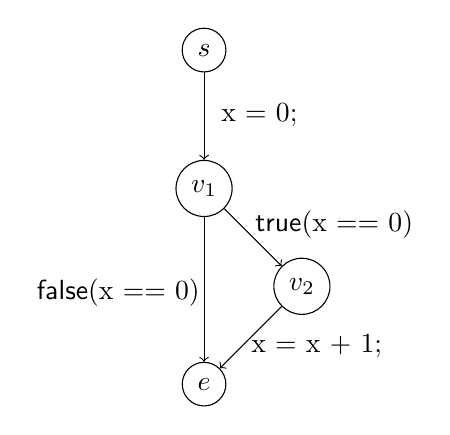
\begin{tikzpicture}[node distance={50pt}, main/.style = {draw, circle}] 
      \node[main] (0) {$s$};
      \node[main] (1) [below of=0] {$v_1$};
      \node[main] (2) [below right of=1] {$v_2$};
      \node[main] (3) [below left of=2] {$e$};
      \draw[->] (0) -- node[midway, xshift=20pt, yshift=16pt, pos=1] {x = 0;} (1);
      \draw[->] (1) -- node[midway, xshift=19pt, yshift=15pt, pos=1] {\textsf{true}(x == 0)} (2);
      \draw[->] (2) -- node[midway, xshift=35pt, yshift=8pt, pos=1] {x = x + 1;} (3);
      \draw[->] (1) -- node[midway, xshift=-31pt, yshift=25pt, pos=1] {\textsf{false}(x == 0)} (3);
    \end{tikzpicture}
  \end{subfigure}
  \caption{Example program (left) and corresponding CFG (right)}
  \label{fig:example_cfg}
\end{figure}

  \section{Static Analysis}
  Static analysis is defined by Rival~\cite{rival2020introduction} as "[...]an automatic technique that approximates in a conservative manner semantic properties of programs before their execution". This means that the program is analyzed just by the given source code without execution. The goal is to prove certain properties about the program in a "sound" manner i.e. any property that is proven to hold actually does hold. However, from failing to prove a property one cannot conclude that the given property does not hold.\\
  In order to prove properties, e.g. finding that a program does not contain races or identifying dead code, we need to gain information about the program. This is done by performing various kinds of analyses. We will focus on flow sensitive analyses from now on i.e. analyses which find properties of the program dependent on the location within it. The semantic of these will be introduced in the following chapters.
  
    \subsection{Flow sensitive analysis}

    As noted above flow sensitive analyses find properties of the program dependent on the point within the program. Expressed differently this means a flow sensitive analysis will find an overapproximation of states the program may be in for any given point within the program or "program point". This state can describe many things dependent on the analysis performed.\\
    First let us define what a program point is: Imagine a control flow graph (CFG), where nodes represent points between instructions within the program. Edges are labeled with instructions or checks (from now on collectively called "actions") and describe the transitions between these points (see example \ref{fig:example_cfg}). Then any node on this CFG would be what we call a program point.\\
    Concretely let $N$ be the set of all program points. Furthermore, let $\mathbb{D}$ be a Domain containing abstract states describing concrete states of the program. This means that some $d \in \mathbb{D}$ can describe many states the program can be in.\\ 
    Then an analysis is expected to find a mapping $\eta: N \rightarrow \mathbb{D}$ which maps program points to abstract states describing that location within the program i.e. for $[n] \in N$, $\eta\ [n]$ should be an abstract state describing all possible states (and possibly more) the program can be in at program point $[n]$.\\
    \\
    As an example we will introduce a values-of-variables analysis for integers. This analysis finds a mapping from a set of variables $X$ to abstractions of their possible values at any given program point. In the scope of this thesis we will focus on abstracting integer values by sets of integers. Thereby the goal of our values-of-variables analysis is to find a mapping $X \rightarrow 2^\mathbb{N}$ for each program point.\\
    Combining this with the semantic of flow sensitive analysis from before, we get that the Domain $\mathbb{D}_\textsf{v}$ for the values-of-variables analysis should be $\mathbb{D}_\textsf{v} = X \rightarrow 2^\mathbb{N}$. Finally, the resulting $\eta_\textsf{v}: N \rightarrow \mathbb{D}_\textsf{v}$ for this analysis describes a mapping $\eta_\textsf{v}\ [n]$ for some program point $[n] \in N$, where $\eta_\textsf{v}\ [n]\ x$ is a set containing all values $x \in X$ may possibly hold at $[n]$. From this we can conclude that $x$ cannot hold any value outside $\eta_\textsf{v}\ [n]\ x$ at program point $[n]$.

    \subsection{Constraint systems}
    We now formulate a way in which we can describe an analysis in the form of constraints. For this we need a partial ordering $\sqsupseteq$ on the domain $\mathbb{D}$.\\
    Then we create a system of constraints which can be solved for a solution. Consider the edges $(u, A, v)$ of the CFG, where each edge denotes a transition from program point $[u]$ to program point $[v]$ via the action $A$. Now let each of these edges give raise to a constraint
    \[\eta\ [v] \sqsupseteq [\![A]\!]^{\#}\ (\eta\ [u])\]
    where $[\![A]\!]^{\#}$ denotes the abstract effect of the action $A$ defining our analysis. In addition, we need a start state. This is given by $\textsf{init}^{\#}: \mathbb{D}$ which is defined depending on the analysis. This gives raise to the start constraint $\eta\ [s] \sqsupseteq \textsf{init}^{\#}$.\\
    \\
    % TODO: Summarize analysis equations
    We will show these ideas with our example of the values-of-variables analysis: Let us define the partial ordering $\sqsupseteq_\textsf{v}$ that will be used in the constraints. We will do this by saying that a mapping $M_1 \in \mathbb{D}_\textsf{v}$ is ordered above another mapping $M_2$ iff for every variable the set it is mapped to in $M_1$ is a superset of the one the variable is mapped to in $M_2$. Formulated formally this is:
    \[M_1, M_2 \in \mathbb{D}_\textsf{v}: M_1 \sqsupseteq_\textsf{v} M_2 \Longleftrightarrow \forall x \in X: M_1\ x \supseteq M_2\ x\]
    Next we define the start state $\textsf{init}^{\#} = M_\top$ for this domain as the mapping that maps every variable to the full set of integers $\mathbb{N}$ i.e. $\forall x \in X: M_\top\ x = \mathbb{N}$. This is because we assume variables to be randomly initialized in our toy language.\\
    It remains to define the abstract effect of actions $[\![A]\!]^{\#}_\textsf{v}$ for our values-of-variables analysis. We will just show the effect of a simple variable assignment:
    \[ [\![ x=y; ]\!]^{\#}_\textsf{v}\ M = M \oplus \{x \mapsto (M\ y) \} \]
    where $M \oplus \{x \mapsto s\}$ denotes that the mapping $M$ is updated such that $x$ will be mapped to the set $s$. The full definition of abstract effects of a values-of-variables analysis can be found at <// TODO>.\\
    % TODO: ref something for full description? Appendix?

    \subsection{Interprocedural analysis}
    So far we only have defined how a program without procedure calls is analyzed. Now we want to introduce procedure calls of the form $f()$. Since a call has its own set of local variables to work with and a call stack can contain multiple of the same procedure (e.g. for recursion), we will analyze procedures in their own environment. However, we need to also consider global variables that may be affected by the analysis. The idea is to give procedures their own starting states and analyze them similarly as we have done before. The final state of the called procedure is then used to be combined back into the state of the caller before the call. Formalized for an edge $(u, f();, v)$ this looks as follows:
    \[\eta\ [s_f] \sqsupseteq \textsf{enter}^{\#}\ (\eta\ [u]) \]
    \[\eta\ [v] \sqsupseteq  \textsf{combine}^{\#}\ ((\eta\ [u]), (\eta\ [e_f])) \]
    where $[s_f]$ and $[e_f]$ are the start and end node of the CFG for procedure $f()$. The functions $\textsf{combine}^{\#}: \mathbb{D} \times \mathbb{D} \rightarrow \mathbb{D}$ and $\textsf{enter}^{\#}: \mathbb{D} \rightarrow \mathbb{D}$ are defined by the analysis. $\textsf{enter}^{\#}$ handles computing the start state or "calling context" for $f()$, while $\textsf{combine}^{\#}$ describes in what way the caller state and the end state of the callee are merged after the call.\\
    It is worth mentioning at this point that even though a procedure can be called from multiple points within the program we still only analyze the procedure once. For $n$ procedure calls $(u_n, f();, v_n)$ we get $n$ constraints for $[s_f]$: $\eta\ [s_f] \sqsupseteq \textsf{enter}^{\#}\ (\eta\ [u_n])$. We can express this differently in a single constraint as follows:
    \[ \bigsqcup \{ \textsf{enter}^{\#}\ (\eta\ [u_n]) | \forall [u_n] \}\]
    where $\bigsqcup$ is the least upper bound i.e. the least $d \in \mathbb{D}$ according to the ordering $\sqsupseteq$ that is ordered above all of its argument elements.\\
    This behavior of only analyzing the procedures once with the least upper bound of all calling contexts is what we call "context insensitivity". It is quite efficient but at the same time not very precise.\\ 
    \\
    For our values-of-variables analysis we will show how $\textsf{enter}^{\#}_\textsf{v}$ and $\textsf{combine}^{\#}_\textsf{v}$ are defined. We need to take global variables into account when computing the calling context and combining after the call. Therefore, we define the two functions as follows:
    \[\textsf{enter}^{\#}_\textsf{v}\ M = M|_{Globals} \oplus \{x \mapsto \mathbb{N} | \forall x \in X\}|_{Locals_\textsf{ce}} \]
    \[\textsf{combine}^{\#}_\textsf{v}\ (M_\textsf{cr}, M_\textsf{ce}) = M_\textsf{cr}|_{Locals_\textsf{cr}} \oplus M_\textsf{ce}|_{Globals} \]
    where $M|_{Locals}$ and $M|_{Globals}$ refers to the mapping $M$ restricted to only the local or global variables respectively. Note that $Locals_\textsf{ce}$ refers to the locals of the callee while $Locals_\textsf{cr}$ refers to the locals of the caller.\\
    To explain these two function let us first look at $\textsf{enter}^{\#}_\textsf{v}$. This function takes the part of the mapping from the caller that contains information about global variables and adds the information of uninitialized local variables used in the procedure to the state. For $\textsf{combine}^{\#}_\textsf{v}$ the local part from the callee is kept, but it is updated with the global part of the callee return state as this contains the updated information about global variables after the procedure call.\\
    % TODO: concrete example of enter from multiple contexts?
    % TODO: describe precision loss here already?

    \subsection{Context sensitivity}

    \subsection{Partial context sensitivity}

    \subsection{Precision loss}
    
  



